\documentclass[psamsfonts,oneside]{amsbook}
\usepackage{nameref}
\usepackage{graphicx}
\usepackage{alltt}
\usepackage[colorlinks]{hyperref}

\newcounter{CellID}[section]
\renewcommand{\theCellID}{\thesection.\arabic{CellID}}

\newenvironment{code}%
{\begin{quote}\refstepcounter{CellID}\ttfamily(* Cell \theCellID{} *)\\\noindent}%
{\rmfamily\end{quote}}

\newcommand{\cellref}[1]{Cell \ref{code:#1}}

\newcommand{\chapref}[1]{Chapter \ref{#1}, ``\nameref{#1}''}

\newcommand{\MReturn}[1]{$\hookrightarrow$ #1}

\newcommand{\expr}[1]{\ttfamily{#1}\rmfamily}

\newcommand{\MPlot}[3]{
	\begin{figure}[t]
	\centering
	\includegraphics{figures/{#1}/{#2}}
	\caption{#3}
	\label{fig:#1_#2}
	\end{figure}
}



\makeindex

\begin{document}
\frontmatter
\title[\emph{Mathematica} for Undergraduate Research]{A Simple Introduction to \emph{Mathematica} for Undergraduate Research Projects}
\author[Jator]{Samuel N. Jator}
\author[French]{Robert D. French}
%\maketitle
\begin{titlepage}
\begin{center}
% Upper part of the page
\textsc{\LARGE An Introduction to}\\[1.5cm]
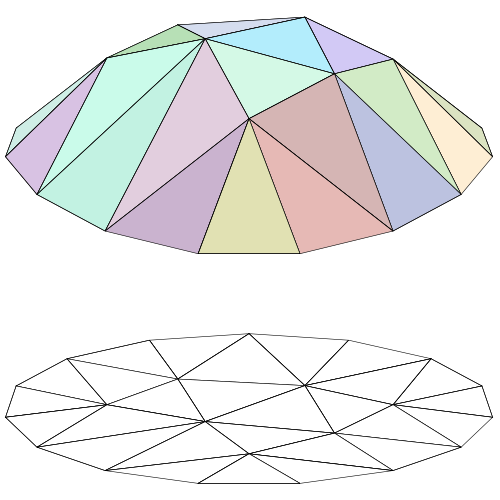
\includegraphics[width=0.5\textwidth]{figures/CustomCover/500px-Piecewise_linear_function2D.png}\\[1cm]    
{ \huge \bfseries \emph{Mathematica} Programming}\\[0.4cm]
\textsc{\Large for Undergraduate Research}\\[0.5cm]
% Title
% Author and supervisor
\begin{minipage}{0.4\textwidth}
\begin{flushleft} \large
Robert D. French
\end{flushleft}
\end{minipage}
\begin{minipage}{0.4\textwidth}
\begin{flushright} \large
Dr.~Samuel Jator
\end{flushright}
\end{minipage}
\vfill
% Bottom of the page
{\large \today}
\end{center}
\end{titlepage}

\tableofcontents
\input{Prependices/Preface}
\chapter*{If you have never used \emph{Mathematica} \ldots }
\label{chap:Prelim}

This pamphlet assumes you have done at least a little programming before, possibly in C, C++, FORTRAN, Visual Basic, or some other language. If not, \emph{that is completely fine}. We will walk you through some simple programming concepts here so that you can get your feet wet, and then you will be ready to take on chapter 1.

If you have done some programming before, but have never used \emph{Mathematica}, it will still benefit you to spend some time with this section, because it will walk you through some tricks to make using \emph{Mathematica} more pleasant.

\section{Notebooks and Cells}
\label{sec:NotebooksAndCells}
When you start \emph{Mathematica} for the first time, it will create a new \emph{notebook} for you. A notebook is just a type of document, like a Microsoft Word document, but it is specially designed to make \emph{Mathematica} programming easier.\footnote{Note that for most programming languages, you type your code in a \emph{plain text} document, or one that has no special formatting in it. This is not the case in \emph{Mathematica}; if you open a notebook in Vim or Notepad, you will see that your code is surrounded by lots of formatting directives that you probably don't want to type by hand!} Notebooks are broken into cells, which you can think of like paragraphs. Each cell can have code in it, and they can be evaluated\footnote{To ``evaluate'' some code simply means to run it.} independently.

You can create new cells by clicking in a blank region of the docoument. You will see the cursor displayed sideways, and that is \emph{Mathematica}'s way of telling you that the cursor is in between cells or that it is not inside a cell. As soon as you start typing anything, a new cell will be created, your cursor will hop inside, and anything you type will be displayed there.

Cells can have different ``Styles'' depending on what you want to use them for. By default, when a new cell is created it will be an ``Input'' cell, which means you can type code in it and evaluate it. By right-clicking on the vertical bar on the right side of a cell, you can bring up a menu that will allow you to change the style of the cell. Changing your cell style to ``Title'', ``Section'', ``Subsection'', etc. as appropriate can help you organize your work and will make your presentations look more professional.

When you type some code in a cell, you can evaluate it by pressing ``Shift+Enter''\footnote{In case you are not familiar with this convention, it means to hold the ``Shift'' key and then press the ``Enter'' button}. In this book, the result of evaluations will be displayed next to a $\hookrightarrow$ symbol. For example:

\begin{code}
	   \label{code:FirstCellEver}
	   5 + 7\\
	   \MReturn{12}
\end{code}

In \emph{Mathematica}, the results of your computation will be displayed in an \emph{output cell} that is attached to the input cell you just evaluated, so it is important to note that we present things in a slightly more compact fashion. Also, you will notice that the above cell is labelled \cellref{FirstCellEver} because it is the first cell in Section \ref{sec:NotebooksAndCells}. Likewise, the next cell will be labelled \cellref{SecondCellEver}:

\begin{code}
	   \label{code:SecondCellEver}
	   cellnumber = 2;\\
	   ``This is the '' <> ToString[cellnumber] <> ``nd cell!''\\
	   \MReturn{``This is the 2nd cell!''}
\end{code}

Please feel encouraged to follow along by typing the code you see here into a \emph{Mathematica} notebook and evaluating them. Much like mathematics, you cannot learn any programming language simply by reading a book -- you must also solve problems and tinker with examples.

\section{Fancy Typing and the Palette}

When you start \emph{Mathematica}, it should load a set of buttons in a thin vertical window to the right of your notebook. If it does not, you can access this palette by going to ``Window'' $\rightarrow$ ``Palettes'' $\rightarrow$ ``Basic Math Input'' in the menu bar. The palette gives you ways to make your code look more mathematical. For example, there are buttons for writing integrals, summations, exponents, matrices, greek letters, etc\footnote{Indeed, many of the basic features of \LaTeX are available in \emph{Mathematica} to help you typeset mathematical expressions, but you will still need the full power of \LaTeX in order to prepare your research for publication.}. If you press any of these buttons, it will insert the necessary symbols into the current cell and you will see several small boxes in the positions where one would expect symbols. Pressing ``Tab'' will allow you to move between these boxes, and type any valid \emph{Mathematica} expression in them.

\subsection{Subscripts, Exponents, and Fractions}

There are also keyboard shortcuts for many of the symbols in the palette. For example, to type a fraction, you can press ``Ctrl+/'' and your cursor will automatically be placed in the numerator. To type the fraction $\frac{2}{3}$ in \emph{Mathematica}, you simply need to press ``Ctrl+/'' and then ``2'', ``Tab'' (which moves you to the denominator), and then ``3''.

Likewise, to type $x^3$, you simply type ``x'' and then ``Ctrl+6'' and then \emph{Mathematica} will give you a black box above and to the right of the ``x'' character and move your cursor there. Then type ``3'', and you will have $x^3$.

You can of course combine elements in expression boxes. For example, to write $x^{\frac{2}{3}}$, you can type ``x'' and then ``Ctrl+6'' to get an expression box in the exponent position, then type ``Ctrl+/'' to turn that box into a fraction, then hit ``2'', ``Tab'', and then ``3''.

\subsection{Greek Symbols (Things like $\pi$, $\theta$, and $\alpha)$}

Using the ``Esc'' button, you can generate these symbols. ``Esc+pi+Esc'' will get you the $\pi$ symbol. You can look at Table \ref{tab:GreekLettersTable} to see a longer list of symbols. These symbols are also available in the ``Basic Math Input'' palette.

\begin{table}
	   \centering
	   \begin{tabular}{ll}
			 Symbol & \emph{Mathematica} code \\
			 $\pi$ & ``Esc'' pi ``Esc'' \\
			 $\alpha$ & ``Esc'' alpha ``Esc'' \\
			 $\beta$ & ``Esc'' beta ``Esc'' \\
			 $\theta$ & ``Esc'' theta ``Esc'' \\
			 $\phi$ & ``Esc'' phi ``Esc'' \\
			 $\eta$ & ``Esc'' eta ``Esc'' \\
			 $\chi$ & ``Esc'' chi ``Esc'' \\
	   \end{tabular}
	   \caption{A table of greek letters}
	   \label{tab:GreekLettersTable}
\end{table}

\subsection{Sums, Integrals, and Derivatives}

These are best accessed by using the corresponding buttons in the ``Basic Math Input'' palette. For example, clicking on the large capital Sigma will give you a summation sign with two input boxes below it and one above. You can type expressions in these boxes and press ``Tab'' to go to the next. You can also construct integrals and derivatives in this fashion. Here are some things to try:

\begin{enumerate}
	   \item Find the sum $\sum_{n=1}^{10} 2^n$
	   \item Make \emph{Mathematica} show you that $\int_0^{\pi} \sin(x) dx = 1$
	   \item Find the derivative of $\sin(x)$
\end{enumerate}

\section{Functions}
\emph{Mathematica} has tons of built-in functions. It has trig functions like \expr{Sin} and \expr{Cos}. It also has functions for plotting graphs and generating lists or tables of data (see ``\nameref{chap:Plotting}'' and ``\nameref{chap:ListsMap}''). In addition, you can create your own functions, but that will be discussed in Chapter \ref{chap:Functions}, ``\nameref{chap:Functions}''. For now, it is important to go over a few basics about how functions work in \emph{Mathematica}.

For example, we know from trig that $\sin(\frac{\pi}{2}) = 1$. To see this for yourself in \emph{Mathematica}, type the following into a cell:

\begin{code}
	   Sin[$\frac{\pi}{2}$]
\end{code}
and press ``Shift+Enter'' to evaluate the cell. Below, you will see an output cell generated containing the number 1. However, there are other functions in \emph{Mathematica} aside from normal math functions. For example, you can use the \expr{Map} function to produce a list of sine values for a given set of domain points. 

To see what we are talking about more clearly, let's consider the set $\{0, \frac{\pi}{2}, \pi, \frac{3\pi}{2}, 2\pi\}$. We can calculate the corresponding range values very simply by applying \expr{Sin} to these values via \expr{Map}.

\begin{code}
	   \label{code:MappedSine}
	   Map[Sin, \{0, $\frac{\pi}{2}$, $\pi$, $\frac{3\pi}{2}$, $2\pi$\}]\\
	   \MReturn{$\{0, 1, 0, -1, 0\}$}
\end{code}
where the $\hookrightarrow$ on the last line indicates the return value from \cellref{MappedSine}.

\section{Variables} 
\emph{Mathematica}'s variables are very simple. Variables can hold numbers, lists, matrices, functions, symbols, or graphs. For now, we will just look at how to store some numbers as variables and see how it affects a plot.

\begin{code}
	   \label{code:PlottedSine}
	   Amplitude = 1;\\
	   UpperBound = 10;\\
	   Plot[Amplitude * Sin[x], \{x, 0, UpperBound\}]
\end{code}

\MPlot{Preliminaries}{SineWithAmplitudeAndUpperBound}{\expr{Sin[x]} on $[0,10]$}

When you execute this, you will see that $\sin(x)$ will be drawn on the interval $[0,10]$, as depicted in Figure \ref{fig:Preliminaries_SineWithAmplitudeAndUpperBound}. Try doing the following by changing the values for \expr{Amplitude} and \expr{UpperBound} in \cellref{PlottedSine}:

\begin{enumerate}
	   \item Plot $2\sin(x)$ on $(0,10)$
	   \item Plot $-\sin(x)$ on $(0,10)$
	   \item Plot $\pi\sin(x)$ on $(0, 2 \pi)$
\end{enumerate}


\mainmatter
\chapter[Stuff You've Seen Before]{A Review of Some Stuff You've Probably Seen Before}
\label{chap:SeenBefore}

Before beginning this chapter, it is assumed that you know a few things about programming already. Specifically, you will need to know how to
\begin{enumerate}
	   \item assign values to variables
	   \item evaluate \emph{Mathematica} cells
\end{enumerate}
and if you don't, that's quite alright. Just see the section ``\emph{\nameref{chap:Prelim}}'' on page \pageref{chap:Prelim}, and even if you have done a bit of programming before, we will walk you through some basic \emph{Mathematica}.

\section{Variable Assignment}
The first thing we need to know in any language is how to assign variables. Probably you are thinking ``\emph{I learned this in CSCI 1010!}'', but \emph{Mathematica} is a subtle language, and does not always work as you might expect if you are coming from C++ or FORTRAN.

\begin{code}
	i = 1;\\
	j = 2\\
	k := 3;\\
	l := 4
\end{code}

Looking at this example, we can see that there are four slightly different ways to ``assign'' values to a variable, so let's discuss this a bit. If you put this code into a \emph{Mathematica} cell, you will see that, upon evaluating the cell, it will output \expr{2}.

So, if we assigned four numbers to four variables, why do we only see one output? The are two key items here. One is the semicolon (;) at the end of the first and third lines. This tells \emph{Mathematica} to suppress the output of that calculation. Generally, it is appropriate to put a semicolon at the end of every line of code in a cell except for the last one. This is because you \emph{usually} want to group your code into cells in such a way that each cell achieves one result, computes one item (or related set of items), or builds one data structure. When debugging, it can sometimes be handy to remove individual semicolons in order to investigate whether each line behaves as you expect.

The second key item is the \expr{:=} operator. This is called the \emph{Set Delayed} operator. This is different from the \expr{=} operator\footnote{also called the \emph{Set} operator} in one important way: it does not assign the value to that variable immediately. Rather, it tells \emph{Mathematica} to wait until \expr{k} or \expr{j} is used and then evaluate the right hand side of that expression. 

What that means, in terms of the above example, is that, at the moment of evaluation, \expr{i} and \expr{j} are numeric variables that contain the values 1 and 2, but \expr{k} and \expr{l} are just symbols that do not yet contain any value. This might be hard to see with the previous example, so let's look at one that's slightly more involved:

\begin{code}
	   \label{code:SetVersusSetDelayed}
	   i = 1;\\
	   j = i + 10\\
	   k := i + 10
\end{code}

When we evaluate this code, we see that the output is simply \expr{11}\footnote{Using what we discussed earlier, can you figure out why this is? See problem 1}. Now we set up a short experiment: We create a few separate cells, and examine what happens to \expr{j} and \expr{k} when we change the value of \expr{i}.

\begin{code}
	   \label{code:SetVersusSetDelayed2}
	   \{j,k\}
\end{code}

\begin{code}
	   \label{code:SetVersusSetDelayed3}
	   i = 2;\\
	   \{j,k\}
\end{code}

\begin{code}
	   \label{code:SetVersusSetDelayed4}
	   i = 20;\\
	   \{j,k\}
\end{code}

\begin{code}
	   \label{code:SetVersusSetDelayed5}
	   i = x;\\
	   \{j,k\}
\end{code}

When we evaluate these cells, we note that they each produce an ordered pair (also called a \emph{list}) as output. This is just to help us see what happens to \expr{i} and \expr{j} when we change the value of \expr{i}.

In \cellref{SetVersusSetDelayed2}, nothing interesting happens. We note that \expr{i} and \expr{j} are both \expr{11} like we expected them to be. But now let's evaluate \cellref{SetVersusSetDelayed3} and see what happens. The output from \cellref{SetVersusSetDelayed3} tells us that \expr{j} is still \expr{11}, but that \expr{k} has been updated to reflect the new value of \expr{i}. This is because the definition we gave for \expr{k} in \cellref{SetVersusSetDelayed} is re-evaluated \emph{every time} we use \expr{k} in an expression.

If we evaluate \cellref{SetVersusSetDelayed4}, we see the same thing has happened: \expr{j} is still \expr{11}, but \expr{k} is now \expr{30}, reflecting the fact that we changed the value of \expr{i} again.

When you evaluate \cellref{SetVersusSetDelayed5}, you will see that is does something slightly different. The explaination is simple, but we leave it as an exercise so that you are forced to think about it!

Delayed Evaluation is most frequently used when defining functions (See \nameref{chap:Functions}). For now, this is as far as we need to go with this topic. You might be thinking: ``\emph{Then why did we even bother?!}'' but, the misuse of this operator is the cause of many bugs, and much of the \emph{Mathematica} code you are likely to find on the internet contains a wild \expr{:=} when it shouldn't. Straightening this out now will spare you headaches, and will promote friendship between you and your code.

\section{Invoking Functions}
\label{sec:InvokingFunctions}

In \emph{Mathematica}, the \emph{invocation operator} is \expr{[]}. This means that, given a function \expr{F}, you can invoke it on an argument \expr{x} by writing \expr{F[x]}. If you do not use the invocation operator, your function will be treated like a variable. Let us look at how this works in a few different scenarios:

\begin{code}
	   Cos[0]\\
	   \MReturn{1}
\end{code}

This is an example of invoking the \expr{Cos} function directly for a single argument. If we want to evaluate \expr{Cos} for a list of arguments, we can instead treat it as a variable and pass it as an argument to the function \expr{Map}:

\begin{code}
	   Map[Cos, \{0, 0.1, 0.2, 0.3, 0.4, 0.5\}]\\
\end{code}

Evaluating this cell will give you all of the values for \expr{Cos} for the domain points $\{0, 0.1, \dots, 0.5\}$. The difference here is that we did not invoke the \expr{Cos} function directly, but rather we passed it as a variable to the \expr{Map} function, which applied \expr{Cos} in turn to each of the data points in our list. 
Some functions are \emph{listable}, which means that when passed a list, they automatically act on each element of the list separately. For example, all of the built-in trig functions are listable, so instead of using \expr{Map} as we have above, we could instead write:

\begin{code}
	   Cos[\{0, 0.1, 0.2, 0.3, 0.4, 0.5\}]
\end{code}

Taking advantage of listable functions allows you to write code that is more elegant and compact\footnote{As with anything, it is possible to go overboard with this technique and write code that is utterly incomprehensible. Use it when it makes sense, and avoid it when you think it might be confusing. Code that is easy to read will win you the respect of peers and professors alike.}. Many other arithmetic operations are also listable, like addition, multiplication, and exponents. 

We can put the famous trig identity $\sin^2(\theta) + \cos^2(\theta) = 1$ to the test with the following code\footnote{It is worth your while to play around with this code until it ``clicks'' for you.}:

\begin{code}
	   \label{code:SineSquaredPlusCosineSquared}
	   thetaValues = \{0, $\frac{\pi}{4}$, $\frac{\pi}{2}$\};\\
	   $\text{Sin[thetaValues]}^2 + \text{Cos[thetaValues]}^2$\\
	   \MReturn{$\{1,1,1\}$}
\end{code}

Of course, not all functions are listable, and sometimes using this feature can make your code harder to read and thus debug. That is why \expr{Map} is a trustworthy alternative. 

{\bf Exercises}. 
\begin{enumerate}
	   \item Explain why the code in \cellref{SetVersusSetDelayed} produces only the single output of \expr{11}
	   \item Explain why \cellref{SetVersusSetDelayed5} produces \expr{\{11,x + 10\}} as an output.
	   \item Explain, using as much detail as you can, what is happening in \cellref{SineSquaredPlusCosineSquared}.
	   \item Think about scalar multiplication and vector addition from Linear Algebra. Do you think these operations could be expressed as listable functions in \emph{Mathematica}? Why or why not?
\end{enumerate}

\chapter[Kernel, State, Scope]{The Kernel, Variable State, and Scope}
\label{chap:Kernel}

Before beginning this chapter, it is assumed that you know a few things about \emph{Mathematica} programming already. Specifically, you will need to know how to
\begin{enumerate}
	   \item assign values to variables
	   \item evaluate \emph{Mathematica} cells
\end{enumerate}
and if you don't, that's quite alright. Just see the section ``\emph{\nameref{chap:Prelim}}'' on page \pageref{chap:Prelim}, and even if you have done a bit of programming before, we will walk you through some basic \emph{Mathematica}.

\section{What is the Kernel?}

In \emph{Mathematica}, all of your coding is done in a \emph{notebook}, and all of the output of your code is displayed there as well. However, the calculations themselves are done in \emph{an entirely separate program}\footnote{This is an example of a Service in a Service Oriented Architecture, and if you are interested in software engineering, you should check this out.}, and this program is called a \emph{kernel}. There are many reasons for doing these calculations in a separate program from your notebooks:

\begin{enumerate}
	   \item You can still edit your notebooks while long computations are running
	   \item You can share variables and data between notebooks
	   \item You can manage multiple kernels, (and thus multiple long-running computations) from a single notebook
	   \item You can run computations on multiple kernels \emph{on other computers}
\end{enumerate}

So we see that this separation of kernel and notebook is very powerful. But what does it mean in terms of your research? Specifically, while you are working on your code, the values you calculate and the variables you assign them to will be stored in your ``Local Kernel''. This assignment of values to variables is called ``State'', and it's just a fancy computer science term for ``The values of your variables at a given time''.

Most of the time, these are just technical points that can be ignored, but understanding how the kernel works will make all the difference in the world when you begin to debug your research program.

\subsection{Quitting the Kernel}. This is kindof like an emergency reset for your program. Quitting the Kernel will basically erase the values for all the variables in your notebook (because they are stored in this separate program which you are about to quit). For example, open a new notebook and evaluate the following code:

\begin{code}
	   (* Cell 1 *)\\
	   NumEggs = 5
\end{code}

Now, in a new cell, evaluate this code:

\begin{code}
	(* Cell 2 *)\\
	Print[``There Are '' <> ToString[NumEggs] <> `` eggs in a Programmer's Dozen''];
\end{code}

And \emph{Mathematica} will display the text ``There are 5 eggs in a Programmer's Dozen''\footnote{As opposed to 13 in a ''Baker's Dozen``}. Now go up to the menu and select ''Kernel`` $\rightarrow$ ''Quit Kernel`` $\rightarrow$ ''Local``. This will cause the kernel you are using to go away, and your variable state will go away with it. Now re-evaluate Cell 2 and see what you get. It will tell you that there are ''NumEggs`` in a Programmer's Dozen. Wait\ldots What?

What's happening here is that when \emph{Mathematica} tries to find a value for the variable \expr{NumEggs}, it notices that one does not exist, so in order to keep your code from exploding\footnote{which is what would happen in other dynamic languages like Ruby or PHP} a value is fabricated for you. The value given is a \emph{symbol object}, which is just a placeholder, kinda like a string, which corresponds to the name ``NumEggs''.

Symbols will be discussed in more detail in Chapter \ref{chap:Symbols}, but for now they aren't important. The thing to focus on here is that the variable \expr{NumEggs} no longer contains the value \expr{5} because you quit the kernel in which it was stored.

\subsection{Debugging with a Secondary Notebook}. When dealing with large \emph{Mathematica} projects, it can sometimes be handy to play around with a particular line of code, or analyze the output from one section before going on to the next cell. You could do this all in one notebook, but that could get sloppy, and you run the risk of messing up some code that is already working\footnote{Although, you are protecting yourself from code loss by using version control, right? If not, check out Appendix \ref{chap:GitHub}, ``\nameref{chap:GitHub}''}.

For example, let's suppose you have the following block of code that does not appear to be working correctly:

\begin{code}
	   (* Cell 3 *)\\
	   EvaluateDerivativeAtAPoint[f\_,x\_] := Block[\{fPrime\}\footnote{Using \expr{Block} is just a way to tell \emph{Mathematica} that \expr{fPrime} should be treated as a \emph{local} variable, which means its value will not be seen outside of the \expr{Block} statement. More on this in Section \ref{sec:Scope}, ``\nameref{sec:Scope}''}, \\
	   	fPrime = f';\\
		fPrime[x]\\
	   ];\\
		\\
	   (* Cell 4 *)\\
	   EvaluateDerivativeAtAPoint[Sin, $\pi$]\\
	   $\rightarrow$ -1\\
	   \\
	   (* Cell 5 *)\\
	   EvaluateDerivativeAtAPoint[$x^2 + x$, $\pi$]\\
	   $\rightarrow$ ($x + x^2$)'[$\pi$]
\end{code}

Why does it give the right answer for $\sin$ but some weird expression for $x^2 + x$? Well, let's open a new notebook and play around with a couple of things. You can open a new notebook by going to ``File''$\rightarrow$``New'' or pressing ``Ctrl+N''. In the new notebook, type the following code:

\begin{code}
	   (* Cell 1 -- Second Notebook *)\\
	   f = $x^2 + x$;\\
	   fPrime = f';\\
	   fPrime[$\pi$]\\
	   $\rightarrow$ ($x + x^2$)'[$\pi$]
\end{code}

The idea here was to repeat the basic logic of our \expr{EvaluateDerivativeAtAPoint} function to see if we could reproduce the problem, and indeed we have. It looks like maybe the third line is not invoking the function? Or maybe the second line is not taking the derivative for some reason? One way to settle that is to remove the third line and then see what happens:

\begin{code}
	   (* Cell 1 -- Second Notebook *)\\
	   f = $x^2 + x$;\\
	   fPrime = f'\\
	   $\rightarrow$ ($x + x^2$)'
\end{code}

Okay, so that looks a little funny, but we remember that it gave the right answer for $\sin$, right? So let's duplicate this cell\footnote{you can click on the bar on the right side of the cell to select it, hit ``Ctrl-C'' to copy, and then ``Ctrl-V'' to duplicate the contents into a new cell.} and try again with \expr{Sin} just to make sure:

\begin{code}
	   (* Cell 2 -- Second Notebook *)\\
	   f = Sin;\\
	   fPrime = f'\\
	   $\rightarrow$ Cos[\#1] \&
\end{code}

My goodness, what is happening here? It is not obvious from looking at it, but that is shorthand \emph{Mathematica} syntax for a new function. It is equivalent to writing \expr{Function[x,Cos[x]]}, which simply means \emph{``Here is a new function that takes x as an argument and gives Cos[x] as its value''}. This will be covered in more detail in Chapter \ref{chap:Functions}, ``\nameref{chap:Functions}'', but for now we don't have to worry about the specifics. 

We can make a guess that maybe, for some reason, the \expr{'} operator won't work on plain expressions like $x^2 + x$, but it will work on things that \emph{Mathematica} recognizes as full-fledged functions like \expr{Sin} and \expr{Cos}. So, how do we make \emph{Mathematica} recognize $x^2 + x$ as a function? Let's try using \expr{Function} to define our expression as a proper function of the variable \expr{x}:

\begin{code}
	   (* Cell 3 -- Second Notebook *)\\
	   f = Function[x, $x^2 + x$];\\
	   fPrime = f'\\
	   $\rightarrow$ Function[x, 1 + 2x]
\end{code}

And we can see now that we have \expr{Function[x, 1 + 2x]} as our result, which means \emph{``Here is a new function that takes x as an argument and gives 1 + 2x as its value''}, and indeed this is what we want for the derivative of $x^2 + x$. Now let us re-introduce the line of code we removed earlier:

\begin{code}
	   (* Cell 3 -- Second Notebook *)\\
	   f = Function[x, $x^2 + x$];\\
	   fPrime = f';\\
	   f'[$\pi$]\\
	   $\rightarrow$ $1 + 2\pi$
\end{code}

So now we understand the nature of the bug: it wasn't that our \expr{EvaluateDerivativeAtAPoint} function was wrong, rather it was that we were invoking it with the wrong \emph{type} of argument. We gave it the \emph{expression} $x^2 + x$ when in fact we should have given it the \emph{function} \expr{Function[x, $x^2 + x$]}. Now we can go back to our first notebook and correct the code in Cell 5:

\begin{code}
	   EvaluateDerivativeAtAPoint[Function[x, $x^2 + x$], $\pi$]\\
	   $\rightarrow$ $1 + 2\pi$
\end{code}

and now we are in good shape. Using this debugging strategy, we were able to fool around with fixing the bug in one notebook without messing up the code in our main notebook. This is an excellent habit, and it will save you mountains of trouble.

\section{Scoping Variables with \expr{Block}}
\label{sec:Scope}

Whenever you use a new variable in  \emph{Mathematica}, the kernel makes a new entry for that variable in the global symbol table. This can be a hassle when debugging, because you may want to re-evaluate a cell over and over while you change it, and sometimes values from previous calculations can sneak in and mess up your code. For example, let's say that you are building a list of intermediate expressions for some larger calculation. Maybe you have to calculate the value of a function and its derivative at certain points and store them in a list\footnote{This may seem like a silly example, but it is one of the first steps in deriving BDF, Numerov, or Adams-style ODE solvers}:

\begin{code}
	   (* Cell 1 *)\\
	   PointsForFunction = \{0, 1, 2\};\\
	   PointsForDerivative = \{3, 4\};\\
	   ListOfValues = \{\};\\
\end{code}
	   
\begin{code}
	   (* Cell 2 *)\\
	   f = Function[x, $x^2 + x$];\\
	   AppendTo[ListOfValues, Map[f, PointsForFunction]]\\
	   $\rightarrow$ \{0, 2, 6\}\\
\end{code}
	   
\begin{code}
	   (* Cell 3 *)\\
	   fPrime = Function[x, $2x$];\\
	   AppendTo[ListOfValues, Map[fPrime, PointsForDerivative]]\\
	   $\rightarrow$ \{0, 2, 6, 6, 8\}\\
\end{code}

Which looks all well and good, except we put the wrong derivative for \expr{fPrime}! Let's fix that and re-evaluate Cell 3:

\begin{code}
	   (* Cell 3 *)\\
	   fPrime = Function[x, $2x + 1$];\\
	   AppendTo[ListOfValues, Map[fPrime, PointsForDerivative]]\\
	   $\rightarrow$ \{0, 2, 6, 6, 8, 7, 9\}\\
\end{code}

Hmmm\ldots that can't possibly be right. It seems like we have too many values here, don't you think? Let's re-evaluate Cell 3 again and see if it does the same thing:

\begin{code}
	   (* Cell 3 *)\\
	   fPrime = Function[x, $2x + 1$];\\
	   AppendTo[ListOfValues, Map[fPrime, PointsForDerivative]]\\
	   $\rightarrow$ \{0, 2, 6, 6, 8, 7, 9, 7, 9\}\\
\end{code}

Okay, it looks like our list is growing by 2 units every time we run this cell. What could possibly be going on? Let's re-evaluate Cell 2 and see what we get:

\begin{code}
	   (* Cell 2 *)\\
	   f = Function[x, $x^2 + x$];\\
	   AppendTo[ListOfValues, Map[f, PointsForFunction]]\\
	   $\rightarrow$ \{0, 2, 6, 6, 8, 7, 9, 7, 9, 0, 2, 6\}\\
\end{code}

Probably, clever reader, you have figured out the bug by now -- Every time we re-evaluate Cells 2 and 3, new values are added to our \expr{ListOfValues}, but we never bothered to reset it, so it just kept growing! 

Now, how do we resolve such a puzzle? The answer is that we can use the \expr{Block} function to keep our variables contained to just one region of the code. That will allow us to re-run cells over and over while we make adjustments, and \emph{Mathematica} will automatically reset the variables for us each time. Check this out:

\begin{code}
	   (* Cell 4 *)\\
	   PointsForFunction = \{0, 1, 2\};\\
	   PointsForDerivative = \{3, 4\};\\
	   ListOfValues = Block[\{temporaryList\},\\
		temporaryList = \{\};\\
		f = Function[x, $x^2 + x$];\\
		AppendTo[temporaryList, Map[f, PointsForFunction]];\\
	   	fPrime = Function[x, $2x + 1$];\\
	   	AppendTo[temporaryList, Map[fPrime, PointsForDerivative]];\\
	   	temporaryList\\
	   ]\\
	   $\rightarrow$ \{0, 2, 4, 7, 9\}
\end{code}

You can re-run that as many times as you like, and you'll never have to worry about values from old calculations sneaking into your list.

\chapter{Defining Your Own Functions}
\label{chap:Functions}

Defining one's own functions is very easy in \emph{Mathematica}. For example, suppose you want a function that converts from Cartesian coordinates to polar coordinates. This is a map of the form $(x,y) \mapsto (r, \theta)$ using the relationships $x = r\cos(\theta)$ and $y = r\sin(\theta)$. We also want an inverse function of the form $(r, \theta) \mapsto (x,y)$ that will convert Polar coordinates to Cartesian. Let's see how this would look in code:

\begin{code}
	   (* Cell 1 *)\\
	   CartesianToPolar[\{x\_,y\_\}]:= \{$\sqrt{x^2 + y^2}$, ArcSin$\left[\frac{y}{\sqrt{x^2 + y^2}}\right]$\};\\
	   PolarToCartestian[\{r\_,$\theta$\_\}]:= \{r Cos[$\theta$], r Sin[$\theta$]\};\\
\end{code}

We can invoke these functions by using the \expr{[]} operator, as discussed in the section ``\nameref{sec:InvokingFunctions}''. Let's see what happens when we do. 

\begin{code}
	   (* Cell 2 *)\\
	   CartesianToPolar[\{1,1\}]\\
	   $\hookrightarrow$ \{$\sqrt{2}, \frac{\pi}{4}$\}\\
\end{code}

Since these two functions are one another's inverse, we can compose them and recover our original input:

\begin{code}
	   (* Cell 3 *)\\
	   point = \{1,1\};\\
	   PolarToCartesian[CartesianToPolar[point]];\\
	   $\hookrightarrow$ \{1, 1\}\\
\end{code}


\section{Using \expr{Block} for Scope}

Notice how, in the above definition of \expr{CartesianToPolar}, we calculate $x^2 + y^2$ in two different places. This isn't the end of the world, but it's a little inelegant, so let's clean it up by calculating it first and using it later as a variable:

\begin{code}
	   (* Cell 4 *)\\
	   CartesianToPolar[\{x\_,y\_\}]:= (\\
	   	r = $\sqrt{x^2 + y^2}$;\\
	   	\{r, ArcSin$\left[\frac{y}{r}\right]$\}\\
	   );\\
\end{code}

That looks much nicer. Cleaning up the code in this way will make your code more readable, and that will make it easier to debug and share with others. However, there is a small side effect: the value stored in \expr{r} will ``leak'' out of your function. To see what this means, let's do an example:

\begin{code}
	   (* Cell 5 *)\\
	   CartesianToPolar[{1,1}];\\
	   r\\
	   $\hookrightarrow$ $\sqrt{2}$
\end{code}

Now, why should \expr{r} even exist outside of where it is defined in the \expr{CartesianToPolar} function? That's because \emph{Mathematica} makes all new variables \emph{global} by default. This means that unless you indicate otherwise, variables created anywhere in your program will be accessible from anywhere else. Global variables are not necessarily bad, but if you don't keep an eye on them they can be a total nightmare.

Fortunately, \emph{Mathematica} provides a construct known as a \emph{block} which allows you to set up some local variables and automatically erase them when you're done. You can make a block by calling the \expr{Block} function like this:

\begin{code}
	   (* Cell 6 *)\\
	   CartesianToPolar[\{x\_,y\_\}]:= Block[{z},\\
			 z = $\sqrt{x^2 + y^2}$;\\
			 \{z, ArcSin$\left[\frac{y}{z}\right]$\}\\
	   ];\\
\end{code}

Now if you repeat the experiment from Cell 5, you will see that no new value is stored in the variable \expr{z}. That is because the block automatically set \expr{z} up as a local variable and erased it when the block ended. Keeping variables like this contained in a block will help keep your code clean, because it will keep cells from adversely interacting with one another. 

\section{Accepting Functions as Arguments}

Frequently it is useful to take a second function as an argument for a function you have defined. There are no specific use cases for this, but if you are familiar with the technique, you will be able to recognize when it will be helpful.

As an example, let's say that you are preparing a report and you would like all of your graphs to be displayed uniformly. You could manually go throuhg your code and set all of your \expr{Plot} settings to be the same, or you could define a single abstract function to take certain arguments and plot all of your graphs in the same style.

Let's assume that in this report, we will be plotting a comparions of \emph{Exact Solutions} versus \emph{Approximate Solutions} for a set of differential equations. That means we want our custom plot function to take two arguments
\begin{enumerate}
	   \item The Exact Solution as a \emph{Mathematica} function
	   \item The Approximate Solution as a list of points to plot
\end{enumerate}
so we know that the \emph{signature} of our function will look like the following:
\begin{code}
	   AwesomePlot[ExactSoln\_, ApproxSoln\_, LowerBound\_, UpperBound\_]:=
\end{code}

This is because we will need to accept not only the Exact Solution and the Approximate Solution, but also the interval on which those solutions should be plotted. This is part of the normal information we would pass to \expr{Plot}\footnote{You may recall that normally \expr{Plot} is invoked by using an expression, not a function variable, as the first argument (i.e. \expr{Plot[Sin[2 x], \{x,0,1\}]}). This is because \expr{Plot} evaluates its arguments in a non-standard way. TODO: List settings. It is defined in such a way that the first argument is ``Held''. TODO: Section on hold evaluations}. Now we want to display both of these functions on the same graph, preferebly in different colors, so that we may compare them. Thus the body of our function may look like:

\begin{code}
	   ExactGraph = Plot[ExactSoln[x], \{x, LowerBound, UpperBound\}, PlotStyle -> Blue];\\
	   \\
	   n = Length[ApproxSoln];\\
	   StepSize = (UpperBound - LowerBound)/(n - 1);\\
	   ApproxPoints = Table[\{ApproxSoln[[i]],(i - 1) * StepSize + LowerBound\},\{i,1,n\}];\\
	   ApproxGraph = ListPlot[ApproxPoints, PlotStyle -> Red];\\
	   Show[ExactGraph, ApproxGraph]
\end{code}

\MPlot{Functions}{AwesomePlotSin}{\expr{AwesomePlot[Sin,\{0,1,0,-1,0\},0,2$\pi$]}}
And we can see that this will form a very handy tool that will make sure all of the plots in your report are very consistent, and it will make your code much, much cleaner.

\section{Recursive Functions}

It is sometimes handy to define a function that turns around and calls itself. This can come up in Math when building recurrence relations, but it can also be a stylistic technique to help keep your code clean and readable. Clever use of recursive functions can make code more concise, and thus more transparent and demonstrable. As stated many other times in this book, code clarity is vital to collaboration.

\subsection{Calculating the Fibonacci Sequence} 

The Fibonacci Sequence is a famous integer sequence that appears unexpectedly in nature and aesthetics. For many, it is the first clue that the world we live in is inherently mathematical. The $n$th term in this sequence, labelled $F_n$, can be calculated as follows:

\begin{align} 
	   F_0 &= 0 \\
	   F_1 &= 1 \\
	   F_n &= F_{n - 1} + F_{n - 2}
\end{align}

Now, how do we build this in \emph{Mathematica}? Notice that in Equation 3, $F_n$ is defined in terms of previous members of the sequence. Let's rephrase these equations in function notation and see if it becomes a little clearer:

\begin{align} 
	   F(0) &= 0 \\
	   F(1) &= 1 \\
	   F(n) &= F(n - 1) + F(n - 2)
\end{align}

So now we can see that the function $F(n)$ \emph{depends on itself}. That is what the notion of a recursive function is all about! So, let's try to build this in \emph{Mathematica}:

\begin{code}
	   (* Cell 1 *) \\
	   F[n\_] := F[n - 1] + F[n - 2];
\end{code}

We can hit ``Shift+Enter'' to evaluate this cell, and we get no complaints from \emph{Mathematica}, so everything must be fine, right? Let's try to calculate \expr{F[2]} and see if we get $1$:

\begin{code}
	   (* Cell 2 *)\\
	   F[2]\\
	   $\hookrightarrow$ \emph{Recursion depth exceeded}
\end{code}

So\ldots that's not cool\ldots But what does that error even mean? It means that our function \expr{F} called itself over and over and over again until \emph{Mathematica} said ``Enough! This thing looks as though it will never stop, so I'm going to stop it for you!''. But why did it not stop at \expr{F[0] = 0} like Equation 4? Well, we didn't tell it when to stop, so when it got to \expr{n = 0}, it called \expr{F[0]} which called \expr{F[-1]} and \expr{F[-2]} and kept right on rolling down into the negative numbers.

That being said, how do we make a recursive function stop at a certain point? As with most things in \emph{Mathematica}, it's pretty easy -- we just tell it when, like this:

\begin{code}
	   (* Cell 1 *)\\
	   F[0] = 0;\\
	   F[1] = 1;\\
	   F[n\_] := F[n - 1] + F[n - 2];
\end{code}

What happens here is that the function \expr{F} actually has different rules that it can execute depending on what the input is. This is the \emph{Mathematica} equivalent of a piecewise-defined function. It is as though we had written:

\begin{align}
	   F(n) = \left\{ \begin{array}{rcl}
			 0 & \mbox{for} & n = 0 \\
			 1 & \mbox{for} & n = 1 \\
			 F(n-1) + F(n-2) & \mbox{for} & n \geq 2
	   \end{array}\right.
\end{align}

When a function has many different rules with different patterns, \emph{Mathematica} will try to match them \emph{in the order they are given}\footnote{Try quitting the kernel and moving line 3 to the top in Cell 1. Re-evaluate the cell and see if you can make a conjecture about why the sequence does not finish in this case.}. The first two rules are expressed without \expr{\_} signs in the arguments. This indicates that they should match exactly the value given. This means the first rule is matched \emph{only} when \expr{n = 0} and it is skipped otherwise.

There are many other types of wilcards, and we will explore these in the next section. It is recommended that you do exercises 5 and 6 before proceeding.

\subsection{Building your own Derivative operator}


\textbf{Exercises}.
\begin{enumerate}
 	   \item In Cell 1, why were the functions defined with their variables inside a list (\{\})? What would be different if the curly braces were le ft off? How would this affect composition in Cell 3?
 	   \item Consider the code given for \expr{AwesomePlot} and explain why \expr{n - 1} yields a more accurate \expr{StepSize} than \expr{n} would. 
	   \item Expand the code for \expr{AwesomePlot} so that it takes a string to use as the title for the plot
 	   \item Expand the code for \expr{AwesomePlot} so that it automatically labels plots as ``Figure 1'', ``Figure 2'', etc without explicitly takin g an argument. Hint: It should contain a variable that gets incremented every time you call \expr{AwesomePlot}. 
	   \item Build a recursive function that can generate the \href{http://en.wikipedia.org/wiki/Fibonacci_word}{Fibonacci Word} of length \expr{n}. 
	   \item Build a recursive function that can test the \href{http://en.wikipedia.org/wiki/Collatz_conjecture}{Collatz Conjecture} for a given Natural number \expr{n}. 
\end{enumerate}

\chapter{Lists, \texttt{Map}, and \texttt{Table}}
\label{chap:ListsMap}
This chapter introduces what computer scientists refer to as \emph{functional programming}. To understand some of the impact of this, we begin by discussing the fundamental data structure of functional programming, the List.

A List is similar to an \emph{array} that you might have encountered in other programming languages. One of the main differences is that Lists are designed to grow, whereas arrays are designed to take up a fixed amount of memory.

Lists in \emph{Mathematica} can be constructed very simply by the following statement:
\begin{code}
	   A = List[];
\end{code}
or equivalently
\begin{code}
	   A = {};
\end{code}
however, the former style should be preferred as it is more explicit\footnote{Good programmers always aim for their code to be \emph{clear} and \emph{explicit}. This makes it easier for others to read their code and understand its meaning, and that is good for friendship}. Lists can be grown by \emph{appending} to elements to them. For example, in order to create the list $1,2,3,4$, we could do the following:
\begin{code}
	   AppendTo[A, 1];
	   AppendTo[A, 2];
	   AppendTo[A, 3];
	   AppendTo[A, 4];
\end{code}

Of course, we could also define this list explicitly as follows:
\begin{code}
	   A = {1,2,3,4};
\end{code}
and this is of course much more concise. Generally, if a list can be defined without doing any calculations, i.e. if it is a constant, you will define it all at once as we have done here. However, if the list must be built up programmatically, it is necessary to use the \texttt{AppendTo} function as described above.

We can also access list elements directly by using the \texttt{[[]]} operator. For example, to get the first element of \texttt{A}, we do as follows:
\begin{code}
	   A[[1]]
\end{code}
Note that unlike most programming languages, \emph{Mathematica} begins indexing lists with \texttt{1} rather than \texttt{0}. This is good, because it is in keeping with most mathematical notation for dealing with vectors and matrices. We can also assign values explicitly to a list by using the \texttt{[[]]=} operator like so:
\begin{code}
	   A[[2]] = 5;
\end{code}

TODO: Can we use DelaySet on a list element? What is the effect of this?

You cannot grow a list in this fashion. That is, for a list like \texttt{A} that has 4 elements, you cannot add a fifth element by 
\begin{code}
	   A[[5]] = 5.0;
\end{code}
This is because, like arrays in C or Java, lists have a fixed width, and \emph{Mathematica} will not allocate more memory for them unless you explicitly tell it to (using the \texttt{AppendTo} function).\footnote{This is a much different model than languages like Perl or Ruby that automatically grow an array when you make an ``out of bounds'' assignment. This strategy, while handy, can slow down your program because memory will be allocated frequently in small chunks rather than infrequently in large chunks.}

\section{The \texttt{Map} Function}

\section{The \texttt{Table} Function}

\section{Vectors, Matrices, and Higher Lists of Lists}

\chapter{Plotting}
\label{chap:Plotting}

\section{Plot}
You can plot $\sin(x)$ on the interval $[0,1]$ with the following \emph{Mathematica} code:
\begin{code}
	   Plot[Sin[x], \{x,0,1\}]
\end{code}
be careful to avoid using the ``;'' on the end of a \texttt{Plot} statement or \emph{Mathematica} will suppress the graphics output and you will not see your plot.

\section{ListPLot}

\section{Plot3D}

\section{3DListPlot}

\chapter{Symbols, Expressions, and Replacement Rules}
\label{chap:Symbols}

\section{Replacement Rules}. When you solve a system of equations \ldots

\section{Transforming Expressions}. You can apply a set of replacement rules to an expression\ldots

\section{Performance Issues}. If part of your code that uses replacement rules seems to be running slowly, you can speed things up by preparing a \emph{dispatch table}.

\appendix
\chapter{Finding Help in \emph{Mathematica} }
\label{chap:Help}

\section{Documentation Center}

You can access \emph{Mathematica}'s built-in documentation center by pressing ``Shift'' + ``F1'' from anywhere in the application. The Help Center provides the official documentation for all fo the built-in functions you will use, and for many additional packages that are included in \emph{Mathematica} but not enabled by default.

Each function has its own page in the Help Center. Try searching for \texttt{Plot}. You will see several things: 
\begin{enumerate}
	   \item A summaray of usage detailing all the ways that \texttt{Plot} can be invoked, and what the differences are.
	   \item A section showing further examples and more sophisticated tricks.
	   \item A list of related functions, such as \texttt{Plot3D} and \texttt{Manipulate}.
\end{enumerate}
One of the difficulties in reading the documentation given in the Help Center is that it references other documentation in the Help Center, and you may get the feeling that you are going in circles. This is quite normal, and no cause for worry. Every programmer encounters this difficulty when learning a new language, though they may not admit it. The trick really is to keep following the trail until you build up enough context that what you are reading starts to make sense.

It is important, in situations like these, to put aside (momentarily) the problem for which you are searching and focus on what is presented in the documentation. Play with the examples that are given. Try changing parts of them, rearranging the arguments, throwing in different numbers or values. If you mess it up, you can always just close the Help Center and come back to it later. Above all, it is vital to \emph{be patient}. 

The single most frustrating experience you can have while programming is to spend ages hunting through the documentation for \emph{The Wrong Way to Do It}. The docs, you see, are designed to show \emph{The Right Way to Do It}, and it may sometimes take a while to recognize that for what it is.

You may trust that the authors have spent many long sessions dumbfounded in front of the \emph{Mathematica} Help Center only to realize in a great flurry of excitement that the answer is completely different than we initially expected. One cannot rush that sort of thing; this stuff just takes time.

\section{Stack Overflow}
One of the greatest resources for \emph{Mathematica} help on the internet is \href{http://stackoverflow.com/questions/tagged/mathematica}{StackOverflow/Mathematica}. Also becoming very popular is \href{http://mathematica.stackexchange.com/}{mathematica.stackexchange.com}, which is a separate site dedicated enitrely to \emph{Mathematica} issues. Both of these should serve you well in your quest to find answers to your problems.

StackOverflow is a forum in which users are encouraged to give insightful answers in order to receive \emph{points}, which amount to social capital. Thus, the answers you will find on StackOverflow are consistently of a higher quality than those you will find on other programming-related websites.

On StackOverflow, all questions are \emph{tagged} according to which programming language or platform they pertain to. The link above will take you directly to the \emph{Mathematica} questions, and from there you can search for more specific information about your question.

Generally, the probability that the issue you have run into when programming in \emph{Mathematica} (or any language) is unique is very low, so the odds are in your favor that someone has encountered a very similar problem before you. Thus, the challenge is to alter your search terms judiciously until you stumble on a problem that seems to fit the issue you are dealing with.

One way to help with this process is to speculate a few guess about what the problem might be. For example, are you using some functions whose behavior you don't quite understand? Maybe you getting a weird output that doesn't look like what you think it should? Searching on StackOverflow for things like ``ListPlot no graph'' is more likely to get you useful results than ``no graph''. 

\subsection{Asking Questions on Stack Overflow}
Accounts on StackOverflow are free, and joining this community will help you learn a great deal about both \emph{Mathematica} and programming in general. Searching through other people's questions and the suggested answers can be very informative, and it is a good intellectual exercise to try to solve some on your own (and you may even be rewarded with profile points!).

Of course, membership on StackOverflow also allows you to post questions. Understand though that the community expects you to have done some work before you post a question. Generally, before posting new questions, it is advisable to:

\begin{enumerate}
	   \item Try your query on a major search engine like Google or Bing. At least try all the links on the first page to see if they have anything helpful to offer.
	   \item Try searching WolframAlhpa. While this is not exactly a search engine in the usual sense, its results usually contain \emph{Mathematica} code which is occasionally helpful.
	   \item Try the \emph{Mathematica} documentation. You can access this by pressing Shift+F1 while running \emph{Mathematica}. Specifically, you will want to look at the examples that are available on the documentation page for each function that you might have questions about. Frequently functions can take different arguments, or give different output depending on parameters or options, so it may be that you need to invoke your function in a slightly different way. 
\end{enumerate}

If you have done these things and still not found the answer to your question, then it will be cool to post your question on Stack Overflow. One thing to note is that while people on Stack Overflow are usually very eager to help, they need enough information about what you are trying to do to be able to understand where you might be running into trouble. Generally, posting a single line of code may not be enough. Also, keep in mind that folks on the internet are very unlikely to be familiar with your research, so it is important to track down the issue as specifically as possible.


\chapter{Using GitHub to Collaborate with Teammates}
\label{chap:GitHub}

If you are working on a research project with a team, you may decide simply to email the mathematica notebooks you are using back and forth every time either of you makes a change. This seems like a good idea, and indeed it is the simplest way to share changes, but it can lead to some surprisingly hairy problems very quickly.

For example, let us suppose that Nell, Ben, and Raman are on a team together. They start with one document, \emph{research1.nb}, which contains all of their initial code that they plan to use for their project, and each person takes a copy of the document home with them. Later that week, Nell and Ben both make separate changes to the document and email their new documents to Raman. When Raman checks her email, she sees that Nell and Ben have both come up with neat ideas, but in order to get them to work together, she has to cut and paste their changes by hand. This seems straightforward enough, until Raman tries to run the code and she encounters a bug!

What might have happened? Did she make a typo while rearranging the code? Do Nell and Ben's changes conflict in some subtle way? Did the documents they emailed her match their latest changes (that is, did either Nell or Ben accidentally send an old document)? Emailing documents leads to many, many difficulties of this nature. Fortunately, programmers before us have encountered this same issue, and developed tools to solve it.

\section{The Value of Version Control}

Version Control is, in general, a way of keeping track of changes to files across a team of people (even if it is only a team of one!). Version Control systems are programs that you can install on your computer that will note the changes you make to your code in a way that allows you to access specific versions of your code at any time.

At first, this may sound like a simple backup system, and version control can certainly act as a backup system, but there are more powerful features than that. For example, version control systems allow you to maintain \emph{multiple histories} of a file. This can be useful when you want to experiment with your code. Nell may be brainstorming an improvement she wants to make to the way that graphs are stored, using a SparseMatrix instead of a List of Lists. With version control, she can ``branch'' from the current development history into a separate \emph{parallel} history so that her experiment will not affect Ben and Raman. If Nell's idea works, she can ``merge'' her branch back into the main history. If it doesn't, she can simply discard it. Either way, it is clear that trying this with a backup system or a set of shared folders would lead to a disorganization nightmare for the team.

\section{Using Git}

Git is an excellent version control system. You can learn how to install it by going to \href{http://git-scm.org}{git-scm.org}. The basic operations in Git are as follows:

\begin{code}
	   \# Creates a new repository
	   \$ git init
\end{code}
Which will create a new repository. The repository is simply the database that keeps track of changes you make to all the files in a given folder. When you make a change to a file, tell Git about it by typing
\begin{code}
	   \$ git add BenNellRaman\_Research.nb
\end{code}
when you have made a set of changes that you would like to be stored in the repository's history, you need to ``commit'' those changes:
\begin{code}
	   \$ git commit -am ``Storage Algorithm now uses SparseMatrix for more efficiency''
\end{code}

\section{Sharing Repositories on GitHub} 

The easiest way to keep a shared repository for your team is for everyone to create an account on \href{http://www.github.com}{GitHub}. GitHub is a free service for hosting open source projects using git. 

TODO setting up repo

TODO giving push access

\chapter{Projects: Building Simple ODE Solvers}
\label{chap:Projects}

\section{Deriving Euler's Method}

\section{Deriving the Improved Euler's Method}

\section{Application of the Methods}

\subsection{Scalar ODEs}

\subsection{Systems of ODEs}

\subsection{Method of Lines and PDEs}

\backmatter
\end{document}
